\documentclass{article}

\usepackage{neurips_2026}
\usepackage[utf8]{inputenc}
\usepackage[T1]{fontenc}
\usepackage{hyperref}
\usepackage{url}
\usepackage{booktabs}
\usepackage{amsfonts}
\usepackage{nicefrac}
\usepackage{microtype}
\usepackage{xcolor}
\usepackage{graphicx}
\usepackage{tikz}
\usetikzlibrary{arrows.meta, positioning}

\title{Gendered Citation Patterns in French Legislative Manifestos (1973--1993)}



\begin{document}

\maketitle

\begin{abstract}
Political manifestos are a window into how candidates construct their political identity and position themselves in the left-right spectrum. This study asks whether male and female candidates in French legislative elections cite political figures differently, with a focus on the gender of cited persons. Using a corpus of 20,331 manifestos from five elections (1973--1993), I build an Natural Languague Processing (NLP) pipeline that extracts person citations via a CamemBERT-NER model and resolves their gender through Wikidata. I find a large and statistically significant gap: female candidates cite women in 44\% of their known-gender citations, compared to 5\% for male candidates (Mann-Whitney $U$, $p < 0.001$). This gap persists across all five election years. Beyond the quantitative difference, the \emph{identity} of cited figures suggests a qualitative distinction: male candidates cite women as electoral actors, while female candidates draw on feminist intellectuals and activists absent from male manifestos. I interpret this as evidence that female candidates actively construct a female political identity, compensating for their low presence in the political scene.
\end{abstract}


%────────────────────────────────────────────────────────────
\section{Introduction}
%────────────────────────────────────────────────────────────

In France, electoral campaigns have long been governed by a legal framework regulating what candidates can communicate and how. During the period studied (1973--1993), among the official tools of electoral communication (\emph{propagande électorale}), there was the \emph{profession de foi}, a campaign document that the state through the \emph{commission de propagande} (a body charged with verifying and distributing electoral materials) printed and sent to every registered voter in the candidate's constituency \cite{gaultier2022}. Crucially, the same rules applied to all candidates regardless of party size, gender, or resources. This uniformity makes \emph{professions de foi} a powerful data source: any differences in content between candidates reflect choices about political identity and positioning, not differences in access or communication capacity.

During this period, female candidacies in France were rare: around 10.6\% of the corpus. Yet the same period coincided with an unprecedented feminist mobilisation: the Mouvement de Libération des Femmes (MLF) was founded in 1970, Gisèle Halimi created \emph{Choisir la cause des femmes} in 1971, and Arlette Laguiller became the first woman to run for the French presidency in 1974 \cite{duchen1986, picq1993}. This wave produced a generation of feminist intellectuals and activists such as Halimi, Laguiller, Huguette Bouchardeau, and Simone de Beauvoir, who became political reference points during the study window.

In this study, I leveraged the Archelec project \cite{gaultier2022}, which has digitised 21,697 \emph{professions de foi} or manifesto documents from five French legislative elections (1973--1993). This paper asks one question in face of the feminist mobilisation: \textbf{Does the gender of cited political figures depend on the gender of the candidate writing the manifesto? And if there is a gap, how big is it?}


%────────────────────────────────────────────────────────────
\section{Related Work}
%────────────────────────────────────────────────────────────

\paragraph{Political manifestos as data:}
Electoral manifestos (\emph{professions de foi}) are a privileged source for studying political identity: unlike speeches or interviews, they are produced systematically by every candidate, enabling large-scale comparison across parties, genders, and election years. The Manifesto Project \cite{merz2016manifesto} demonstrated the analytical value of this source by building a corpus of over 1,800 annotated manifestos across 40+ countries, and prior lexical analyses of French \emph{professions de foi} have mapped candidate positioning from word-frequency patterns \cite{mots2002}. Our work extends this tradition to \emph{citation behaviour}: whose names they invoke, and whether the gender of those figures varies systematically by the gender of the candidate writing the manifesto.

\paragraph{NER for political actor extraction:}
Extracting mentions of political actors from institutional documents via NER is an established approach in computational political science. Kerkvliet, Kamps and Marx \cite{kerkvliet2020} apply NER to Dutch parliamentary proceedings to study who mentions whom, constructing a labelled dataset of political actor spans across party, ministerial, and personal name categories. I follow a similar design applied to historical French manifestos, using \texttt{Jean-Baptiste/camembert-ner} \cite{martin2020camembert}, a CamemBERT model fine-tuned on WikiNER and the French TreeBank, and link the extracted entities to Wikidata for gender resolution.

\paragraph{Gender visibility in political discourse and knowledge bases:}
Research on gendered political discourse has shown that female politicians receive systematically less media coverage than male counterparts, and when covered, face disproportionate attention to appearance and personal life rather than policy \cite{vderpas2020}. A parallel gap exists in structured knowledge bases: Wagner et al.\ \cite{wagner2015} demonstrate that even when women are present on Wikipedia, they are described more through relational and family attributes than professional ones, suggesting that structured data about female figures may be less complete.

\paragraph{Role models and gendered political mobilisation:}
Campbell and Wolbrecht \cite{campbell2006} show that the visibility of female politicians in the media increases adolescent girls' political ambitions, with the effect mediated through family political discussion. Gender gaps in political representation and the under representation of women in the political discourse have been studied extensively \cite{norris1997passages, celis2008, lawless2004}. My work contributes to the role model idea at the text level: I ask which figures female candidates make visible in their own manifestos, and whether doing so might reflect the creation of new role models.

\paragraph{Concurrent work:} Francis \cite{francis2026}\footnote{\url{https://github.com/cynthia-francis/NLP-Gender-Rhetoric-French-Electoral-Manifestos}} applies a Non-Negative Matrix Factorization (NMF) topic modelling to the same Archelec corpus and finds that female candidates emphasise "Gender \& Labor Identity" topics five times more frequently than male candidates, while male candidates default to "Institutional \& Local Development" themes. My analysis complements this topic-level finding by moving to the level of individual named figures, asking whether they construct their political identity by invoking different political actors.

%────────────────────────────────────────────────────────────
\section{Data}
%────────────────────────────────────────────────────────────

\subsection{Archelec Corpus}

As mentioned before, I use the Archelec corpus, a digitised collection of French legislative election manifestos (\emph{professions de foi}) from the French National Archives. I focus on five legislative elections: 1973, 1978, 1981, 1988, and 1993, the years for which digitised text is available. 

\begin{table}[h]
  \label{tab:corpus}
  \centering
  \begin{tabular}{lrrr}
    \toprule
    Year & Total manifestos & Female candidates & \% Female \\
    \midrule
    1973 & 3,768 & 195 & 5.2\% \\
    1978 & 4,794 & 659 & 13.7\% \\
    1981 & 3,115 & 316 & 10.1\% \\
    1988 & 3,455 & 347 & 10.0\% \\
    1993 & 5,199 & 643 & 12.4\% \\
    \midrule
    Total & 20,331 & 2,160 & 10.6\% \\
    \bottomrule
  \end{tabular}
\caption{Corpus composition by election year and candidate gender.}
\end{table}

Of the 21,697 digitised text files, 21,167 matched a metadata record (97.6\%), and the remaining 530 were discarded. After filtering to candidates with a corresponding gender (\emph{homme} or \emph{femme}), the final corpus is \textbf{20,331 manifestos}. Female candidates represent 10.6\% of the corpus overall, with marked variation across years: the share peaked at 13.7\% in 1978 before falling to 10.0--10.1\% in 1981-1988 and recovering to 12.4\% in 1993. Digitisation coverage is identical across genders (100\%), ruling out a sampling bias.

\subsection{Text Quality}

I measured the OCR noise as the ratio of non-alphabetic, non-space characters. It is low and stable across years (mean 0.045). Language detection identifies 97.8\% of manifestos as French, 1.9\% are in English, and 0.16\% in German (Alsace-Moselle). Non-French manifestos are retained but NER performance may be lower on these.

The median manifesto is 963 tokens; 88\% exceed the 512-token limit of CamemBERT-NER, meaning NER covers only the first $\approx$350 words of most texts. I accept this constraint, noting that candidates typically name key political figures early in their manifestos.


%────────────────────────────────────────────────────────────
\section{Methodology}
%────────────────────────────────────────────────────────────

This section describe (1) the full information extraction pipeline (NER + Gender Tagging), and (2) the gender citation share $s_i$ used further in the analysis.

\subsection{Information Extraction Pipeline}

Figure~\ref{fig:pipeline} gives an overview of the full pipeline.

\begin{figure}[h]
\centering
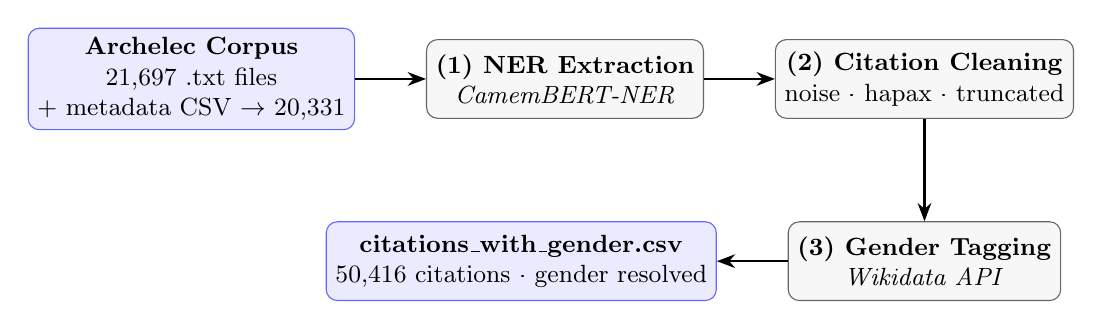
\begin{tikzpicture}[
    node distance=1.3cm and 0.9cm,
    every node/.style={font=\small},
    box/.style={
        rectangle, draw=black!60, rounded corners, fill=gray!6,
        align=center, minimum height=1.0cm, minimum width=2.9cm
    },
    databox/.style={
        rectangle, draw=blue!60, rounded corners, fill=blue!8,
        align=center, minimum height=1.0cm, minimum width=2.9cm
    },
    arrow/.style={-{Stealth}, thick}
]
% Row 1
\node[databox] (input) {
    \textbf{Archelec Corpus}\\
    21{,}697 .txt files\\
    + metadata CSV $\rightarrow$ 20{,}331
};
\node[box, right=of input] (ner) {
    \textbf{(1) NER Extraction}\\
    \textit{CamemBERT-NER}
};
\node[box, right=of ner] (clean) {
    \textbf{(2) Citation Cleaning}\\
    noise · hapax · truncated
};

% Row 2
\node[box, below=of clean] (gender) {
    \textbf{(3) Gender Tagging}\\
    \textit{Wikidata API}
};
\node[databox, left=of gender] (output) {
    \textbf{citations\_with\_gender.csv}\\
    50{,}416 citations · gender resolved
};

% Arrows
\draw[arrow] (input)  -- (ner);
\draw[arrow] (ner)    -- (clean);
\draw[arrow] (clean)  -- (gender);
\draw[arrow] (gender) -- (output);

\end{tikzpicture}

\vspace{0.8em}
\scriptsize
\begin{itemize}
  \item \textbf{85,827} raw citations extracted; \textbf{50,416} retained after cleaning.
  \item Gender resolved for \textbf{66.1\%} of citations via Wikidata (\texttt{wdt:P21}).
\end{itemize}
\caption{Pipeline overview: from raw manifesto texts to citation gender analysis.}
\label{fig:pipeline}
\end{figure}

\subsubsection{Named Entity Recognition}

I extract person citations using \texttt{Jean-Baptiste/camembert-ner}\footnote{\url{https://huggingface.co/Jean-Baptiste/camembert-ner}}, a CamemBERT model fine-tuned on French NER datasets (WikiNER and the French TreeBank). I apply it with \texttt{aggregation\_strategy=``simple''} to merge subword tokens into full entity spans, retaining only \texttt{B-PER} entities with confidence $> 0.7$. Given the research question, I restricted the NER pipeline to PER entities, discarding all other entity types (locations, organisations, dates)

I manually annotated a \href{https://github.com/AnahiRM/NER_gender/blob/main/data/annotation_sample_filled_out.csv}{stratified sample} of 50 manifestos (25 female, 25 male), generating 154 model predictions. Each prediction was marked as correct (TP) or erroneous (FP) and noted missed names (FN). Results for \texttt{B-PER} are:


\begin{table}[h]                                                         
    \centering                                                           
    \begin{tabular}{lr}                                                    
    \hline                                                               
    \textbf{Metric} & \textbf{Value} \\                                  \hline                                                               True Positives (TP)  & 132   \\                                      False Positives (FP) & 22    \\                                      False Negatives (FN) & 3     \\                                      \hline                                                               Precision            & 0.857 \\                                      Recall               & 0.978 \\                                      F1 Score             & 0.913 \\                                      \hline                                                               Precision (femme)    & 0.812 \\
      Precision (homme)    & 0.913 \\                                    \hline                                         
    \end{tabular}  
    \caption{Gender NER evaluation results.}                             \label{tab:ner-eval}
\end{table}

Precision is lower for female-candidate manifestos (0.812 vs.\ 0.913 for male), likely because female manifestos contain more local and non-public figures that the model tags with lower accuracy.

I prefer \texttt{Jean-Baptiste/camembert-ner} over domain-specific alternatives such as \texttt{adminBERT} because the target entities are public political figures, persons prominent enough to appear in Wikipedia, which is precisely the training domain of WikiNER.

\subsubsection{Citation Cleaning}

Raw NER output contains 85,827 citations (38,460 unique names). I apply four cleaning steps:

\begin{enumerate}
  \item \textbf{Noise removal} (4,910): honorifics and titles misclassified as persons (\emph{Monsieur}, \emph{Président de la République}, etc.)
  \item \textbf{Single-token removal} (10,470): one-word spans are too ambiguous to identify reliable figures.
  \item \textbf{Truncated-name removal} (441): names ending in a single character, e.g. "Giscard D'".
  \item \textbf{Hapax removal} (19,590): names appearing only once are likely noise or very local figures.
\end{enumerate}

After cleaning: 50,416 citations, 10,139 unique names.

\subsubsection{Gender Tagging via Wikidata} %CHECK

For each of the 10,139 unique names, I queried the Wikidata MediaWiki API in two steps: (1) \texttt{wbsearchentities} to retrieve candidate Q-IDs, and (2) \texttt{wbgetentities} to verify that the entity is a human (\texttt{wdt:P31 wd:Q5}) and retrieve their sex or gender property (\texttt{wdt:P21}).

The gender was resolved for 5,146 / 10,324 queried names (49.8\%), giving:

  \begin{table}[h]                        
      \centering
      \small                                                                      
      \begin{tabular}{lr}
    \toprule
    Gender & Citations \\
    \midrule
    Male    & 30,995 (61.5\%) \\
    Unknown & 17,073 (33.9\%) \\
    Female  &  2,337 (4.6\%)  \\
    Other   &     11 (0.0\%)  \\
    \bottomrule
\end{tabular}
      \label{tab:gender_dist}                                                     
      \caption{Gender distribution of citations after Wikidata resolution. }                                                             
  \end{table}

The 33.9\% unknown rate could be due to: (1) Wikidata systematically under-representation of women: female figures are less likely to have entries than male figures of equivalent prominence \cite{wagner2015}, and (2) the presence of local and minor figures: candidates' competitors, local councillors, and community organisers.

\subsection{Gender Citation Share}

For each candidate $i$, the female citation share is defined as:
%
\begin{equation}                            
    s_i \;=\; \frac{c_i^f}{c_i^f + c_i^m}                                         
\label{eq:share}                          
\end{equation}     

%   
where $c_i^f$ and $c_i^m$ are the number of citations to female and male figures by candidate $i$. Citations with unknown gender are excluded from both numerator and denominator, so $s_i$ is defined only for candidates with at least one resolved citation. 

%────────────────────────────────────────────────────────────
\section{Results}
%────────────────────────────────────────────────────────────

\subsection{Core Finding: Female Candidates Cite Women Significantly More}

I compare the distributions of $s_i$ across female and male candidates using a one-sided Mann-Whitney $U$ test (non-parametric, robust to the heavily skewed distributions observed). Female candidates cite women nearly nine times more often than male candidates do, and this difference is significant at the 99\% level. 


\begin{table}[h]                                          
    \centering
    \small
    \begin{tabular}{lrr}
    \toprule
    & Female candidates & Male candidates \\
    \midrule
    $N$ candidates & 1,320 & 12,262 \\
    Mean \% female cited & 43.99\% & 4.69\% \\
    \midrule
    \multicolumn{3}{l}{Mann-Whitney $U = 12{,}463{,}618$, $p < 0.001$} \\
    \bottomrule
\end{tabular} 
    \caption{Mann-Whitney $U$ comparing men and women distributions (one-sided, $H_1$: female candidates cite women more than male candidates).}            
    \label{tab:mw}
\end{table}


%The gap of $\approx$39 percentage points is worth diving deep at it, given that female candidates and male candidates cite Mitterrand, Rocard, and Le Pen as their dominant references, so it could be expected that they navigate a similar political rhetoric.




\subsection{Temporal Stability}

The gap is observed across all five election years examined, with female candidate rates ranging from 28\% (1988) to 58\% (1978) and male candidate rates ranging from 2\% (1973) to 7\% (1978). This gap does not close, ranging from 26 to 51 percentage points depending on the year.

\begin{figure}[h]
    \centering                         
    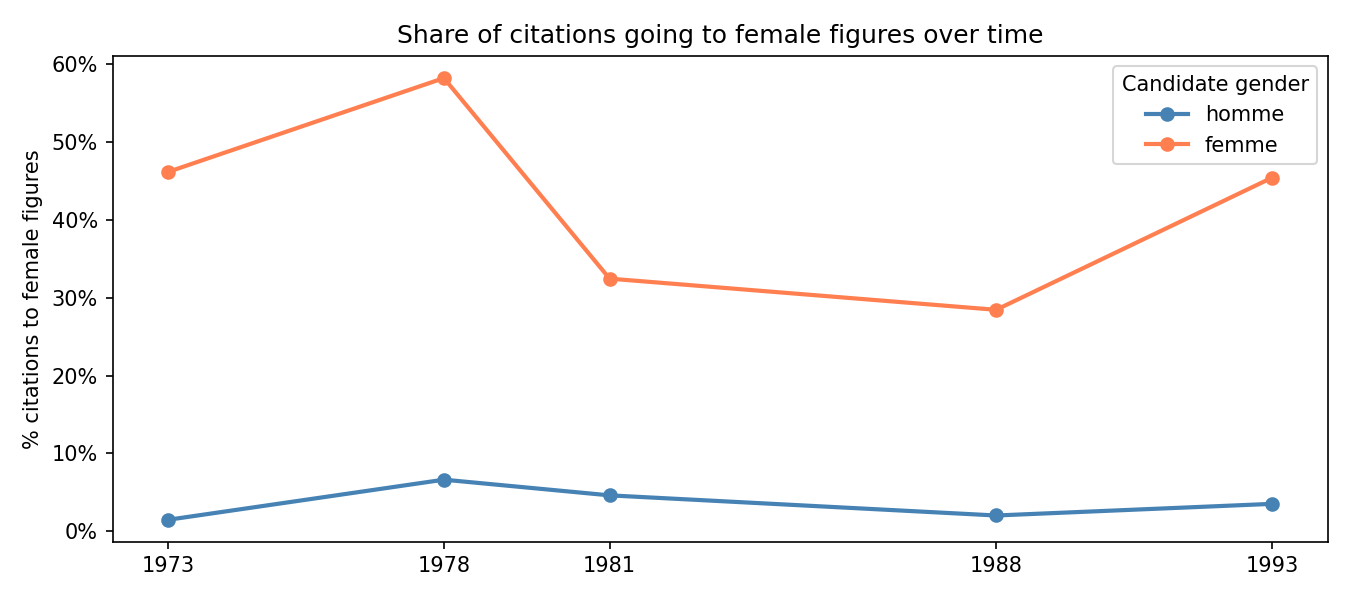
\includegraphics[width=0.7\textwidth]{figures/fig_temporal.png}
    \vspace{0.3em}                      
    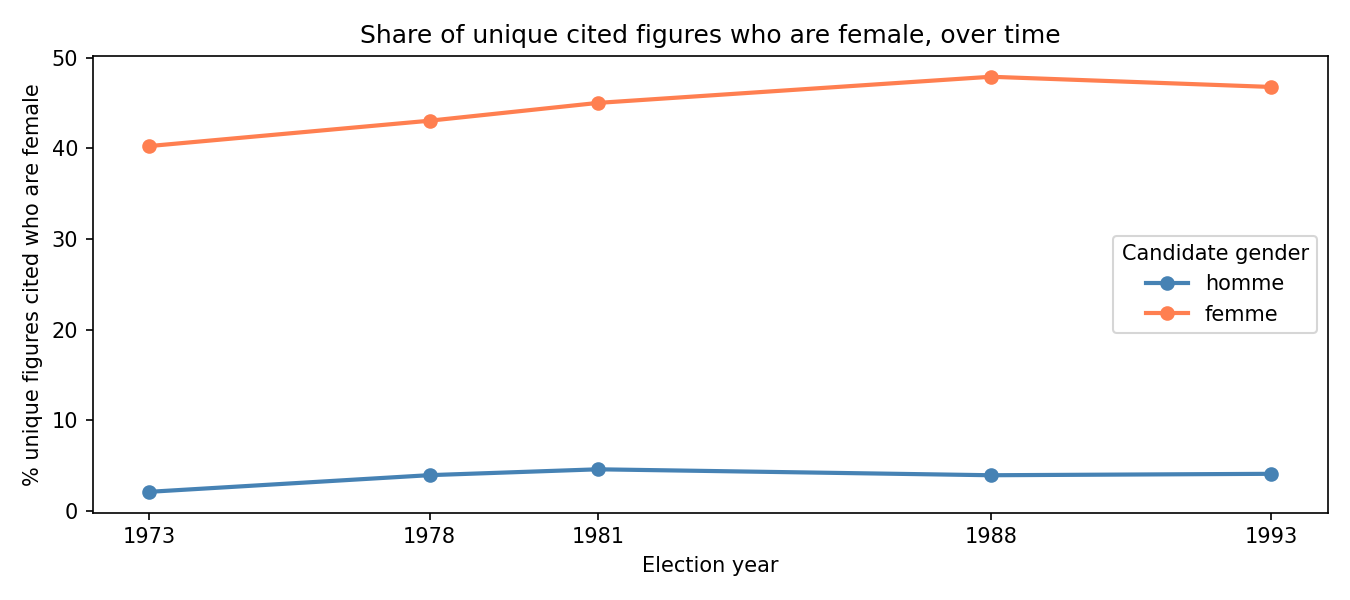
\includegraphics[width=0.7\textwidth]{figures/fig_temporal_figures.png}
    \caption{Top: share of citation events going to female figures, by candidate gender and election year. Bottom: share of unique cited figures that are female, by candidate gender and election year.}
    \label{fig:temporal}                  
\end{figure}  

A complementary analysis of \emph{unique} cited figures suggests an increasing number of female figures for female candidates to cite (40\% in 1973 to 48\% in 1988), while the unique-figure rate for male candidates remains flat between 2\% and 5\%. This indicates that the raw number of citation rates reflect a few women cited repeatedly, rather than a  decline in female citation. Female candidates were modestly broadening the diversity of known women they cited over time.

\subsection{The Qualitative Pattern of Who is Cited}

Both groups share the same dominant references: François Mitterrand (20.5\% of female manifestos, 15.7\% of male), Michel Rocard, and Le Pen. The mainstream political landscape looks the same for both genders. The differences are quantitatively small, but qualitatively relevant.

\begin{table}[h]                                          
    \centering
    \small                                                  
    \label{tab:top20}
    \begin{tabular}{lrlr}                                     
  \toprule                                                                        
  \multicolumn{2}{c}{\textbf{Female candidates}} & \multicolumn{2}{c}{\textbf{Male
   candidates}} \\                            
  \cmidrule(lr){1-2} \cmidrule(lr){3-4}   
  Name & \% & Name & \% \\                    
  \midrule                                                                        
  François Mitterrand       & 20.54 & François Mitterrand      & 15.67 \\
  Arlette Laguiller         & 16.21 & Michel Rocard            &  4.31 \\         
  Michel Rocard             &  5.01 & Le Pen                   &  3.03 \\
  Le Pen                    &  4.33 & Jean-Marie Le Pen        &  2.79 \\         
  De Wendel$^*$       &  4.27 & Arlette Laguiller        &  2.70 \\
  Jean-Marie Le Pen         &  4.21 & Jacques Chirac           &  2.44 \\         
  Brice Lalonde             &  4.15 & Valéry Giscard d'Estaing &  1.85 \\         
  Gisèle Halimi$^*$   &  2.54 & Giscard d'Estaing        &  1.62 \\         
  Jacques Monod$^*$   &  2.48 & Georges Pompidou         &  1.60 \\         
  Jean Rostand$^*$    &  2.48 & Brice Lalonde            &  1.55 \\         
  Simone de Beauvoir$^*$ & 2.48 & Pierre Mauroy$^*$ &  1.23 \\        
  Jacques Chirac            &  1.73 & Raymond Barre$^*$  &  1.22 \\         
  Giscard d'Estaing         &  1.67 & F. Mitterrand            &  1.00 \\         
  F. Mitterrand             &  1.18 & Georges Marchais$^*$ & 0.90 \\        
  André Lajoinie$^*$  &  1.05 & Antoine Pinay$^*$  &  0.90 \\         
  Valéry Giscard d'Estaing  &  1.05 & Robert Fabre$^*$   &  0.71 \\         
  Georges Pompidou          &  1.05 & Président Pompidou       &  0.70 \\         
  Président Pompidou        &  0.99 & Michel Jobert$^*$  &  0.60 \\         
  R. Barre$^*$        &  0.99 & Jean Lecanuet$^*$  &  0.54 \\         
  Huguette Bouchardeau$^*$ & 0.99 & ---                 &    --- \\         
  \bottomrule          
\end{tabular}                                                          
    \caption{Top 20 cited figures by candidate gender (percentage of manifestos   
  citing the figure). Figures marked $^*$ appear in one group's top 20 but not the
   other's.} 
\end{table}

Arlette Laguiller (Lutte Ouvrière, far-left) appears in 16.2\% of female manifestos vs.\ 2.7\% of male. Gisèle Halimi (feminist lawyer), Simone de Beauvoir (feminist philosopher) appear in 2.4\% of female manifestos but are absent from the male top 20. Humanist intellectuals Jacques Monod and Jean Rostand (biologist and philosopher-scientist) also appear exclusively in female candidates' top references. Meanwhile, female candidates cite feminist intellectuals, activists, and advocates, there is only one woman, Arlette Laguiller, that made it to the top 20. The citation gap is therefore not only quantitative but also qualitative: female candidates might use citations to construct a feminist political identity, drawing on a non-electoral intellectual figures as it offers very few female role models.




%────────────────────────────────────────────────────────────
\section{Discussion}
%────────────────────────────────────────────────────────────

My results show that the citation gap existed between 1973 and 1993, reflecting a systematic difference in how male and female candidates constructed their political references. My interpretation is that the low overall female citation rate may be due to the scarcity of prominent female figures in the political environment, rather than male hostile citing women. They operated in a political environment where women had not yet reached the level of national prominence required to become a natural reference point in electoral discourse. The pool of citable female figures was structurally scarce.

To construct the female discourse of the era, female candidates had to reach beyond their electoral sphere. By citing Halimi and Beauvoir alongside Laguiller, they included new female reference points to build a new discourse and its representation in politics. This is consistent with the role model theory of political participation \cite{campbell2006}: female candidates may be using their manifestos to signal to female readers that there is a lineage, a set of women who fought and thought about power, and that political involvement is a legitimate space for women. Connecting my work to the one done by Francis \cite{francis2026}, applying topic modelling to the same corpus, she finds a parallel divergence but at the topic level: female candidates emphasise gender and labour identity themes while male candidates default to institutional references. Together, the two studies suggest that female candidates construct a coherent alternative political identity, in both vocabulary and the figures they cite.

These patterns presented in the results are consistent with the hypothesis that female candidates use citations to navigate a \emph{two-dimensional} political space. Both groups use standard political figures references to signal position on the left-right axis--Mitterrand for the left, Barre or Chirac for the right--and female candidates do this too. But female candidates add a second layer: by invoking Beauvoir, Halimi, or Laguiller alongside standard partisan figures, they might be including figures relevant to women, potentially supporting the feminist discourse of the era. This is consistent with Celis et al. \cite{celis2008}, who argue that female politicians are tasked with representing both a partisan constituency and a gendered one. However, this interpretation is an inference from the political profiles of the cited figures, not from textual analysis of the sentences. Testing it directly by distinguishing strategic identity-construction from incidental co-citation would require sentence-level analysis of manifesto passages, which I leave for future work.

\paragraph{Limitations.}
The three main limitations I faced are the following. First, the 33.9\% unknown gender rate introduces a conservative bias: if unknown citations skew female (as Wikidata's gender gap suggests), the true citation gap is larger than reported. Second, NER covers only the first $\approx$350 words of most manifestos, missing citations in later paragraphs. Third, citation counts are not citation context: I cannot determine from this analysis whether a name is cited approvingly, critically, or neutrally. Fourth, the study period ends in 1993; it would be valuable to extend the analysis to more recent elections, where female candidacy rates have grown substantially.

\paragraph{Additional future work.}
A continuation to my work could comprehend the following. First, a name-based gender classifier (e.g., \texttt{gender\_guesser}) applied to unresolved citations could help to shrink the Wikidata bias. Second, extending the corpus to post-1993 elections would test whether the citation gap narrows as more women enter the political mainstream. Third, sentence-level analysis of citation context would allow us to distinguish symbolic citations (invoked to construct identity) from adversarial ones (cited as rivals to criticise).

%────────────────────────────────────────────────────────────
\section{Conclusion}
%────────────────────────────────────────────────────────────

Female and male candidates in French legislative elections (1973--1993) cohabit a similar political landscape in their manifestos: the same dominant male figures anchor both groups' discourse but differ in the female figures they invoke. Female candidates cite women nearly nine times more often, and the specific figures they choose reveal a deliberate effort to construct a feminist political genealogy. This gap is stable across two decades.

These findings complement the existence of a gender gap in citations with the construction of their political discourse: female candidates were doing something qualitatively distinct with their manifestos, drawing on feminist thought and activism to populate a political world that had structurally excluded them. For women in politics, the manifestos were part of their political identity-making.

\bibliographystyle{unsrt}                                                       
\bibliography{references} 

\appendix

%\input{checklist.tex}

\end{document}
